\section{Introduction}\label{sec:intro}
%\commentt{ CYCLES ARE WONDERFUL; TESTING IS WONDERFUL; Some more concrete points to make:}
Detecting small subgraphs with  specific structures  (referred to as \emph{finding network motifs}) is a basic algorithmic task, with a variety of applications in biology, sociology and network science (see e.g.~\cite{HoLe70, Co88, portes2000social, EcMo02, burt2004structural, milo2002network, alon2007network, foucault2010friend, BerryHLP11, SeKoPi11, JRT12}). 
% \reut{added a couple of examples - is it better than nothing?} \commentt{am adding a few more (from the counting cliques paper, hopefully not in a too superficial manner}
Of special  interest is the natural %\commentt{another word? no word} 
case of subgraphs that are cycles of a fixed size $k$, which we denote by $C_k$.
When the algorithm receives the entire graph as input, then by the well known %\commentt{celebrated?} 
result of Alon, Yuster and Zwick~\cite{AYZ}, this task can be solved in  time $\widetilde{O}(n^{\omega})$ 
% for constant $k$, 
where $n$ is the number of graph vertices and $\omega$ is the exponent of matrix multiplication.\footnote{The dependence on $k$ is exponential, but $k$ is considered a constant.}
But what if we seek a sublinear-time (randomized) algorithm that does not read the entire graph? Namely, the algorithm is given  query access to the graph\footnote{\label{foot:queries} The  types of queries typically considered are neighbor queries (``what is the $i$th neighbor of a vertex $v$?''), degree queries (``what is the degree of a vertex $v$?''), and pair queries (``is there an edge between a pair of vertices $v$ and $u$?'').} % \commentt{Where do we say what are the queries we consider}
and should find a $C_k$ when the graph is not $C_k$-free.
% of a small, constnat size, subgraph, denoted $H$, with high constant probability when the graph is not $H$-free.
This is clearly not possible if the graph contains only a single copy of $C_k$. 
However, is it possible to detect such a copy in sublinear-time when the graph is relatively far from being $C_k$-free?
By ``relatively far'' we mean that it is necessary to remove a non-negligible fraction, denoted $\eps$, of its edges in order to obtain an $C_k$-free graph. %An equivalent 
A closely related formulation of the question is whether we can design a one-sided error algorithm for testing $C_k$-freeness.\footnote{The problems are equivalent if the algorithm is not given access to degree queries, otherwise the algorithm might find evidence to the existence of a $C_k$ without actually detecting one. We note that all our algorithms do detect copies of $C_k$ when they reject.}


If the maximum degree in the graph is upper bounded by a parameter $d_{\max}$, then the $C_k$-freeness testing problem can easily be solved by performing a number of queries that grows polynomially with $d_{\max}$ and exponentially with $\Theta(k)$~\cite{GR-bound}. \commentt{Explain that this holds in general model or no need?}
% $O(d_{\max}^{\ell/2+1}/\eps)$ queries, where $\ell$ is the diameter of $H$. 
In particular, when $d_{\max} = O(1)$, then there is no dependence on the size of the graph $G$. 
% \commentt{this is trivial but I guess we still need to reference GR (bounded-degree paper). or maybe not, since GR worked in a different model} 
We are however interested in considering graphs with varying degrees, so that, in particular, the maximum degree may be   much larger than the average degree, and possibly as large as $\Theta(n)$.
% where $n$ is the number of vertices in $G$.


For the special and interesting case where $k=3$, i.e., the cycle is a triangle,  Alon, Kaufman, Krivelevich and Ron~\cite{AKKR08} gave several upper and lower bounds on the query complexity of testing triangle-freeness as a function of the average degree $d$ of the graph (in addition to the dependence on $n$ and $\eps$).
While the upper and lower bounds are not tight  in general, they are tight for $d=O(1)$, where the complexity is $\Theta(\sqrt{n})$ (for constant $\epsilon$). 
The lower bound in this case is essentially based on ``hiding'' a small clique. 


Since the aforementioned lower bound relies on the existence of a small dense subgraph, a natural question, studied by Levi~\cite{Reut}, is whether it is possible to obtain improved (and possibly tight) results when the arboricity of the graph, denoted $arb(G)$, is bounded.\footnote{The arboricity of a graph $G$ is the minimum number of forests required to cover its edges, and is equal (up to a factor of $2$) to the maximum average degree of any subgraph of $G$.} Focusing on the result under the assumption that $m\geq n$ (i.e., $d= \Omega(1)$) Levi showed that  
$\widetilde{O}(arb(G))$  queries are sufficient for testing triangle-freeness (the dependence on $1/\epsilon$ is polynomial), and that $\Omega(arb(G))$ queries are necessary.\footnote{To be precise, this lower bound holds for $m\geq (arb(G))^3$ -- if $m< (\arg(G))^3$ then the lower bound is $\Omega(m^{1/3})$. \SodaReb{See also Footnote~\ref{foot:loglogn} regarding the upper bound.}}
In particular, when $arb(G)$ is a constant, the complexity is polynomial in $1/\eps$ and does not depend on the size of the graph.




% Our starting point is Levi's work. 
In this work we seek to understand the complexity of testing $C_k$-freeness, in particular with one-sided error, for fixed $k> 3$. Our main focus is on constant arboricity graphs and some of our results extend to bounded arboricity graphs, as well as to $F$-freeness for any general subgraph $F$ (of constant size). 
We note that the problem of testing cycle-freeness
% , in particular with one-sided error, 
without requiring the cycle to be of specific length, is  different from our problem. We further discuss this in Section~\ref{subsec:related}.
In the next subsection we state our findings.



\subsection{Our results}

Since our main focus is on graphs with constant arboricity, we first state our results in this setting, and later discuss our extensions to graphs with non-constant arboricity.
Throughout this paper we assume that $m = \Omega(n)$ since  %the complexity of the algorithm must grow with 
even obtaining a single edge in the graph requires $\Omega(n/m)$ queries. 
Our algorithms use degree and neighbor queries and our lower bounds also allow pair queries (see Footnote~\ref{foot:queries}).
For simplicity, we state our results for constant $\epsilon$. All our algorithms have a polynomial dependence on $1/\eps$, which is stated explicitly in the corresponding technical sections.




Our first finding is that, as opposed to the case of $k=3$, where the complexity of testing $C_3$-freeness grows with the arboricity of the graph but not with the size of the graph,\footnote{We note that this is true also for other $k$-cliques for $k > 3$.} this is no longer the case for $k=4$ (and larger $k$). In particular: 

\begin{theorem}\label{thm:C4-5}
The query complexity of one-sided error testing of $C_4$-freeness in constant-arboricity graphs over $n$ vertices is $\widetilde{\Theta}(n^{1/4})$.
The same bound holds for testing $C_5$-freeness.
\end{theorem}
 The more detailed statements for testing $C_4$ and $C_5$ freeness 
can be found in Theorems~\ref{thm:C4-ub}--\ref{thm:C5-const-alpha-lb}.

Theorem~\ref{thm:C4-5} \ICALPCR{(together with the upper bound in~\cite{GR-bound})}
answers negatively  the following open problem raised by Goldreich.

\smallskip\noindent\textsf{Open problem (number 3.2 in~\cite{goldreich2021open}): From bounded degree to bounded arboricity.} \newline
\textit{Suppose that property $\Pi$ is
testable within complexity $Q(n,\eps)$ in the bounded-degree graph model. Provide an upper
bound on the complexity of testing $\Pi$ in the general graph model under the promise that the tested graph has constant arboricity. For example, can the latter complexity be linear in $Q(n,\eps)$ while
permitting extra $poly(log n)$ or $1/\eps$ factors?}
\smallskip

The $\Omega(n^{1/4})$ lower bound for testing $C_4$-freeness, answers this question negatively. Indeed, %it is easy to show that
testing $C_4$-freeness in $d$-bounded degree graphs  can be done with $poly(d,\eps)$ queries~\cite{GR-bound}, while our lower bound suggest that even in constant  arboricity graphs, a polynomial dependence on $n$ is necessary.
% \fi

\smallskip
When $k \geq 6$, we show that it is no longer possible to obtain a complexity of $\widetilde{O}(n^{1/4})$ as is the case for $k=4,5$.

\newcommand{\GenLB}{
Let $k\geq 6$.
Any one-sided error tester for the property of $C_k$-freeness in graphs of constant arboricity over  $n$ vertices 
must perform $\Omega(n^{1/3})$ queries.
}


\begin{theorem}\label{thm:lb_ck_const_alpha}
\GenLB
\end{theorem}


While for $C_6$ we were not able to match the lower bound of $\Omega(n^{1/3})$, we were able to obtain a sublinear-time algorithm, as stated next.


\begin{theorem}\label{thm:C6-ub-intro}
% \CsixUB
There exists a one-sided error algorithm for testing $C_6$-freeness in graphs of constant arboricity  over $n$ vertices whose query complexity %and running time are
is $\widetilde{O}(n^{1/2})$.
\end{theorem}
% The precise (polynomial) dependence on $1/\eps$ can be found in Theorem~\ref{thm:C6-ub}.
% \commentt{or not say this? }

% \commentt{DR: check exponent - maybe write as $\tilde{O}(n^{1/2})\cdot \poly(1/\eps)$?}
% \talya{in any case I think it shouldnt be stated here}

\smallskip
For general (fixed) $k$ we prove the following upper bound. 





\begin{theorem}\label{thm:Ck-ub-intro}
There exists a one-sided error algorithm for testing $C_k$-freeness in graphs of constant arboricity over $n$ vertices whose query complexity %and running time are 
is $O(n^{1-1/\lfloor k/2 \rfloor })$. 
% \CkUB
\end{theorem}
% \commentt{changed to floor}

\SodaReb{
We also prove a more general result for testing $F$-freeness for any constant size subgraph $F$. Below, $\ell(F)$ is as defined in Definition~\ref{def:ell}, and is always upper bounded by the number of vertices in $F$.}

\begin{theorem}\label{thm:Gen-F-ub-intro}
\SodaReb{There exists  a one-sided error algorithm for testing  $F$-freeness in graphs of constant arboricity over $n$ vertices whose query complexity is $O(n^{1-1/\ell(F)}).$}
\end{theorem}


 \subsubsection{Extensions for general arboricity}


We state our results for general arboricity graphs assuming that the algorithm is given an 
% as a function of $n$, $\epsilon$, and a given
upper bound $\alpha$ on the arboricity of the graph (in  the lower bounds the algorithm may be assumed to know the arboricity).
Alternatively,
if the algorithm receives as an input the number of edges, $m$, (as in previous results for $C_k$-freeness~\cite{AKKR08, Reut}) instead of an upper bound on the arboricity, then we can estimate a notion known~\cite{Reut} as the ``effective arboricity'' of the graph, and depend on it instead of $\alpha$. This is potentially beneficial since the effective arboricity can be much smaller than the actual arboricity of the graph, \SodaReb{and it does not affect the asymptotic running times of our algorithms in terms of the dependence on the size of the graph and $\alpha$}. For further details see Section~\ref{sec:prel}.

For $C_4$-freeness we give both an upper bound and a lower bound for general arboricity graphs. In particular, we show that a linear dependence on $\alpha$ is sufficient and a $\sqrt{\alpha}$-dependence is necessary (both for one-sided error algorithms) as stated next.

\ICALPCR{
\begin{theorem}\label{thm:C4-ub}
There exists a one-sided error algorithm for testing $C_4$-freeness in graphs of arboricity at most $\alpha$ over $n$ vertices whose query complexity  is $\tilde{O}\left(\min\{n^{1/4}\alpha, \alpha+n^{3/4}\}/\eps^3\right)$.\footnote{More precisely, for values $\alpha<\log n$, the complexity is $O(n^{1/4}\alpha^{1/2}\log^{1/2}n/\eps^3)$, for values $\log n < \alpha<\sqrt n$, the complexity is $O(n^{1/4}\alpha/\eps^3)$, and for values $\alpha>n^{1/2}$, it is $O( (\alpha+n^{3/4})/\eps^3)$.}
\end{theorem}


\begin{theorem}\label{thm:C4-gen-alpha-lb}
Testing $C_4$-freeness with one-sided error in graphs over $n$ vertices with arboricity $c_1\log n < \alpha < n^{1/2}/c_1'$ for sufficiently large constants $c_1$ and $c_1'$ requires $\Omega(n^{1/4}\alpha^{1/2})$ queries for constant $\epsilon$.\footnote{Note that the two-sided error lower bound of $\Omega(n^{1/4})$ for constant arboricity graphs (as stated in Theorem~\ref{thm:C4-5}) also holds for graphs with higher arboricity $\alpha$, and in particular, $\alpha = O(\log n)$. This is the case since we can simply add a small subgraph with arboricity $\alpha$ and no $C_4$s to the lower bound construction.} 

\end{theorem}
}

For general
\SodaReb{constant size subgraphs $F$ (and in particular $C_k$)}
our upper bound also has at most a linear dependence on $\alpha$
--
see Theorem~\ref{thm:Gen-F-ub} and Corollary~\ref{cor:Ck-ub} for a precise statement.




We comment that our lower bound of $\Omega(n^{1/3})$  for one-sided error algorithms, $k \geq 6$ and constant arboricity (stated in Theorem~\ref{thm:lb_ck_const_alpha}) also applies to graphs with non-constant arboricity (by adding a $C_k$-free subgraph with  higher arboricity).\footnote{For an odd $k$, it suffices to add a dense bipartite graph, and for even $k$, by the Erd\H{o}s girth conjecture~\cite{E63}, one can add a subgraph with arboricity $n^{2/k}$.} 
 
We also note that it is possible to extend our algorithms for $C_5$ and $C_6$ freeness so as to get a polynomial (but not linear) dependence on $\alpha$. However,  these extensions do not introduce new techniques (and are most probably not optimal), so we do not present them here.







\subsection{A high-level discussion of our algorithms and lower bounds}\label{subsec:high-level-intro}
\ForFuture{reconsider epsilon in this part}
Before discussing each of our results in more detail, we highlight some common themes. The starting point of all our algorithms is that if a graph is $\eps$-far from being $C_k$-free  (for a constant $k$), then it contains $\Omega(\eps m)$ edge-disjoint cycles.\footnote{\ICALPCR{To verify this, let $G$ be a graph that is $\epsilon$-far from being $C_k$-free for a fixed constant $k$. Consider any maximal set $S$ of edge-disjoint $k$-cycles. Since by removing all $k\cdot |S|$ edges on these cycles, the graph can be made cycle-free, $|S| \geq \epsilon m /k = \Omega(\epsilon m)$.}}
We next use the bounded arboricity of the graph. Specifically, if a graph has arboricity at most $\alpha$, then the number of edges between pairs of vertices that both have degree greater than $\theta_0 = \Theta(\alpha/\eps) $, is at most $O(\eps m)$. 

Hence, there is a set of edge-disjoint $C_k$s, which we denote by $\calC$, such that $|\calC| =\Omega(\eps m)$, and no $C_k$ in $\calC$ contains any edge between two vertices with degree greater than $\theta_0$. In other words, for every $k$-cycle $\rho$ in $\calC$, and for every vertex $v$ with degree greater than $\theta_0$ in $\rho$, the two neighbors of $v$ in $\rho$ have degree at most $\theta_0$.
In particular, when $\alpha$ is a constant, the two neighbors have degree $O(1/\eps)$.

At this point our algorithms diverge, but there are two common aspects in the case of $k=4,5,6$ which we would like to highlight. The first is that for the sake of ``catching'' one of the $C_k$s in $\calC$, it will be useful to  consider a subset, $\calC'$, in which every vertex $v$ that participates in one of the edge-disjoint $C_k$s in $\calC'$ actually participate in $\Omega(\eps\cdot d(v))$  $C_k$s in $\calC'$. The existence of such a subset follows by applying (as a mental experiment) a simple iterative process that removes $C_k$s with vertices that do not obey this constraint.

To illustrate why it is useful to have such a set $\calC'$, consider the case of $k=4$, and assume that a relatively large fraction of the $C_4$s in $\calC'$ contain, in addition to the two vertices of degree at most $\theta_0 = O(\alpha/\eps)$, at least one other vertex  that has degree at most $\theta_1=O(n^{1/2}/\eps)$. 
\SodaReb{
In this case we can obtain such a vertex $v$ with high probability (as discussed below), and then sample 
roughly $\sqrt{d(v)/\eps} = O(\sqrt{\theta_1/\eps})=O(n^{1/4}/\eps)$ of its neighbors, so that the following holds.}
By (a slight variant of) the birthday paradox, with high constant probability we hit two of its neighbors, $u$ and $u'$, that reside on the same $C_4$ in $\calC'$ (and hence have degree at most $\theta_0$). By querying all the neighbors of $u$ and $u'$, we obtain this $C_4$.

However, what if for most of the $C_4$'s in $\calC'$ there are two vertices with degree significantly larger than $\sqrt{n}$ (that are ``one opposite the other'' on the $C_4$s)? Roughly speaking, in this case we exploit the fact that the number of such high-degree vertices is bounded, and we show how to detect a $C_4$ by performing random walks of length $2$. A related issue arises in the case of $k=6$, when there are three very high degree vertices on most $C_6$s in $\calC'$. In this case we show how to essentially reduce the problem to testing triangle-freeness in a certain auxiliary graph. 
%
More precisely, the auxiliary graph is a multi-graph to which we have access only to certain types of queries, so that we cannot apply the algorithm of~\cite{AKKR08}. However, we can still show how to obtain a triangle in this graph, and hence a $C_6$ in the original graph. Interestingly, our general lower bound of $\Omega(n^{1/3})$ for $C_k$-freeness, $k\geq 6$ builds on the lower bound for testing triangle-freeness of~\cite{AKKR08}.

% \commentt{I think we should try and start with some ``highlights'' of our ideas before getting into the details. This will require some thought}

\smallskip
In the following subsections we assume for the sake of the exposition that $\eps$ is a constant. 



\subsubsection{The  results for $C_4$-freeness (and $C_5$-freeness)}
We discuss our results for $C_4$-freeness in graphs with general arboricity. 
The results for $C_5$-freeness in constant arboricity graphs are obtained using very similar techniques. 
% \ICALPCR{Recall that we have a one-sided error algorithm whose query complexity $\tilde{O}(n^{1/4}\alpha)$, a lower bound of $\Omega(n^{1/4}\alpha^{1/2})$ for any one-sided error algorithm, and a lower bound of $\Omega(n^{1/4})$ for any two-sided error algorithm for graphs with constant arboricity.}

\paragraph{The algorithm.}
% For the sake of simplicity, assume $\eps$ is a constant (the dependence on $1/\eps$ is polynomial)
% and furthermore, in what follows we ignore constants.
Our algorithm for testing $C_4$-freeness,  \TestCfour, \ICALPCR{which has query complexity $\widetilde{O}(n^{1/4}\alpha)$,}  
is governed by two thresholds: $\theta_0=\Theta(\alpha)$, and $\theta_1=\Theta(n^{1/2})$. 
For the sake of the current high-level presentation, 
%Note that we may 
we 
assume that\footnote{Indeed, graphs with arboricity greater than $n^{1/2}$ necessarily contain at least one $C_4$, but since we are interested in a one-sided error algorithm, and $\alpha$ is only known to be an upper bound on $\alpha$, the algorithm cannot reject if it is provided with $\alpha > n^{1/2}$.} $\alpha \leq n^{1/2}$, 
%since otherwise the graph must contain $C_4$s.
%\commentt{this is not quite precise. If we only have an upper bound on the arboricity, then we can't simply reject}
so that $\theta_0\leq \theta_1$.

The algorithm first samples $O(1)$ edges approximately uniformly by invoking a procedure
\SelectEdge,\footnote{\SodaReb{This is a fairly standard and simple procedure, where we use the fact that graph has bounded arboricity, so that most of its edges have at least one endpoint with degree $\theta_0$.}}
and then randomly selects one of their endpoints. For each vertex $v$ selected, it queries its degree, $d(v)$. If $d(v)\leq \theta_1$, then the algorithm selects $O(\sqrt{d(v)})$ random neighbors of $v$, and for each selected neighbor $u$ such that $d(u)\leq \theta_0$,  it queries all the neighbors of $u$. If $d(v)>\theta_1$, then the algorithm
performs $\widetilde{O}(n^{1/4}\alpha^{1/2})$ random walks of length two from $v$. If a $C_4$ is observed in any one of these steps, then the algorithm rejects, otherwise it accepts.

\paragraph{The analysis of the algorithm.}
By the above description, the algorithm will only reject a graph if it detects a $C_4$, implying that it never errs on $C_4$-free graphs. Hence, consider a graph $G$ that is far from being $C_4$-free. As discussed at the start of Section~\ref{subsec:high-level-intro}, the setting of $\theta_0=\Theta(\alpha)$ (together with the fact that $G$ is $\Omega(1)$-far from being $C_4$-free) implies the following. There exists a set, denoted $\calC$, of $\Omega(m)$ \emph{edge-disjoint} $C_4$s in $G$, such that
 no $C_4$ in $\calC$ contains an edge
% (where $m$ denotes the number of edges in $G$). Furthermore,
% Since the arboricity of $G$ is at most $\alpha$, by the setting of $\theta_0 = \Theta(\alpha)$, the number of $C_4$ that do not contain any edge 
between two vertices that both have degree greater than $\theta_0$. 
Thus, for each $C_4 $ in $\calC$, there are at most two vertices with degree greater than $\theta_0$, and they do not neighbor each other. 
% \talya{perhaps less details since this was already discussed}\commentt{That's true, but need to think how to do it } \talya{Just say recall} \commentt{please check if better}

Considering the second aforementioned  degree threshold $\theta_1$
(and recalling that %we assume here that 
$\theta_1 \geq \theta_0$), we partition $\calC$ into two subsets. The first, $\calC_1$, consists of those $C_4$s in $\calC$ that contain at most one vertex with degree greater than $\theta_1$, and the second, $\calC_2$, of the remaining $C_4$s in $\calC$, which contain exactly two vertices with degree greater than $\theta_1$.
Since $\calC = \calC_1 \cupdot \calC_2$, at least one of these subsets is of size $\Omega(m)$.

\smallskip\noindent\textsf{$C_4$s with at most one high-degree vertex.}
Suppose first that $|\calC_1|=\Omega(m)$. Observe  that since each $4$-cycle $\rho\in \calC_1$ contains at least two vertices with degree at most $\theta_0$ and at most one vertex with degree greater than $\theta_1$, it must contain at least one vertex, with degree at most $\theta_1$ whose neighbors on the $C_4$ both have degree at most $\theta_0$. For an illustration, see the LHS of Figure~\ref{fig:C4-ub}. 
Furthermore, we show that there exists a subset of $\calC_1$, which we denote by $\calC_1'$, such that $|\calC_1'|=\Omega(m)$, and every vertex $v$ that participates in one of the $C_4$s in $\calC_1'$, actually participates in $\Omega(d(v))$ edges-disjoint $C_4$s in $\calC_1$. 
It follows that in this case, when the algorithm selects a random edge (almost uniformly), with high constant probability it will obtain an edge with (at least) one endpoint $v$ having the above properties. Conditioned on the selection of such a vertex $v$,
the algorithm selects $\Theta(\sqrt{d(v)})$ random neighbors of $v$. By the birthday paradox, with high constant probability, among these neighbors there will be a pair of vertices that reside, together with $v$, on a common $C_4$ in $\calC_1'$. Once their (at most $\theta_0$) neighbors are queried, this $C_4$ is revealed.

\begin{figure}[htb!]
\centerline{\mbox{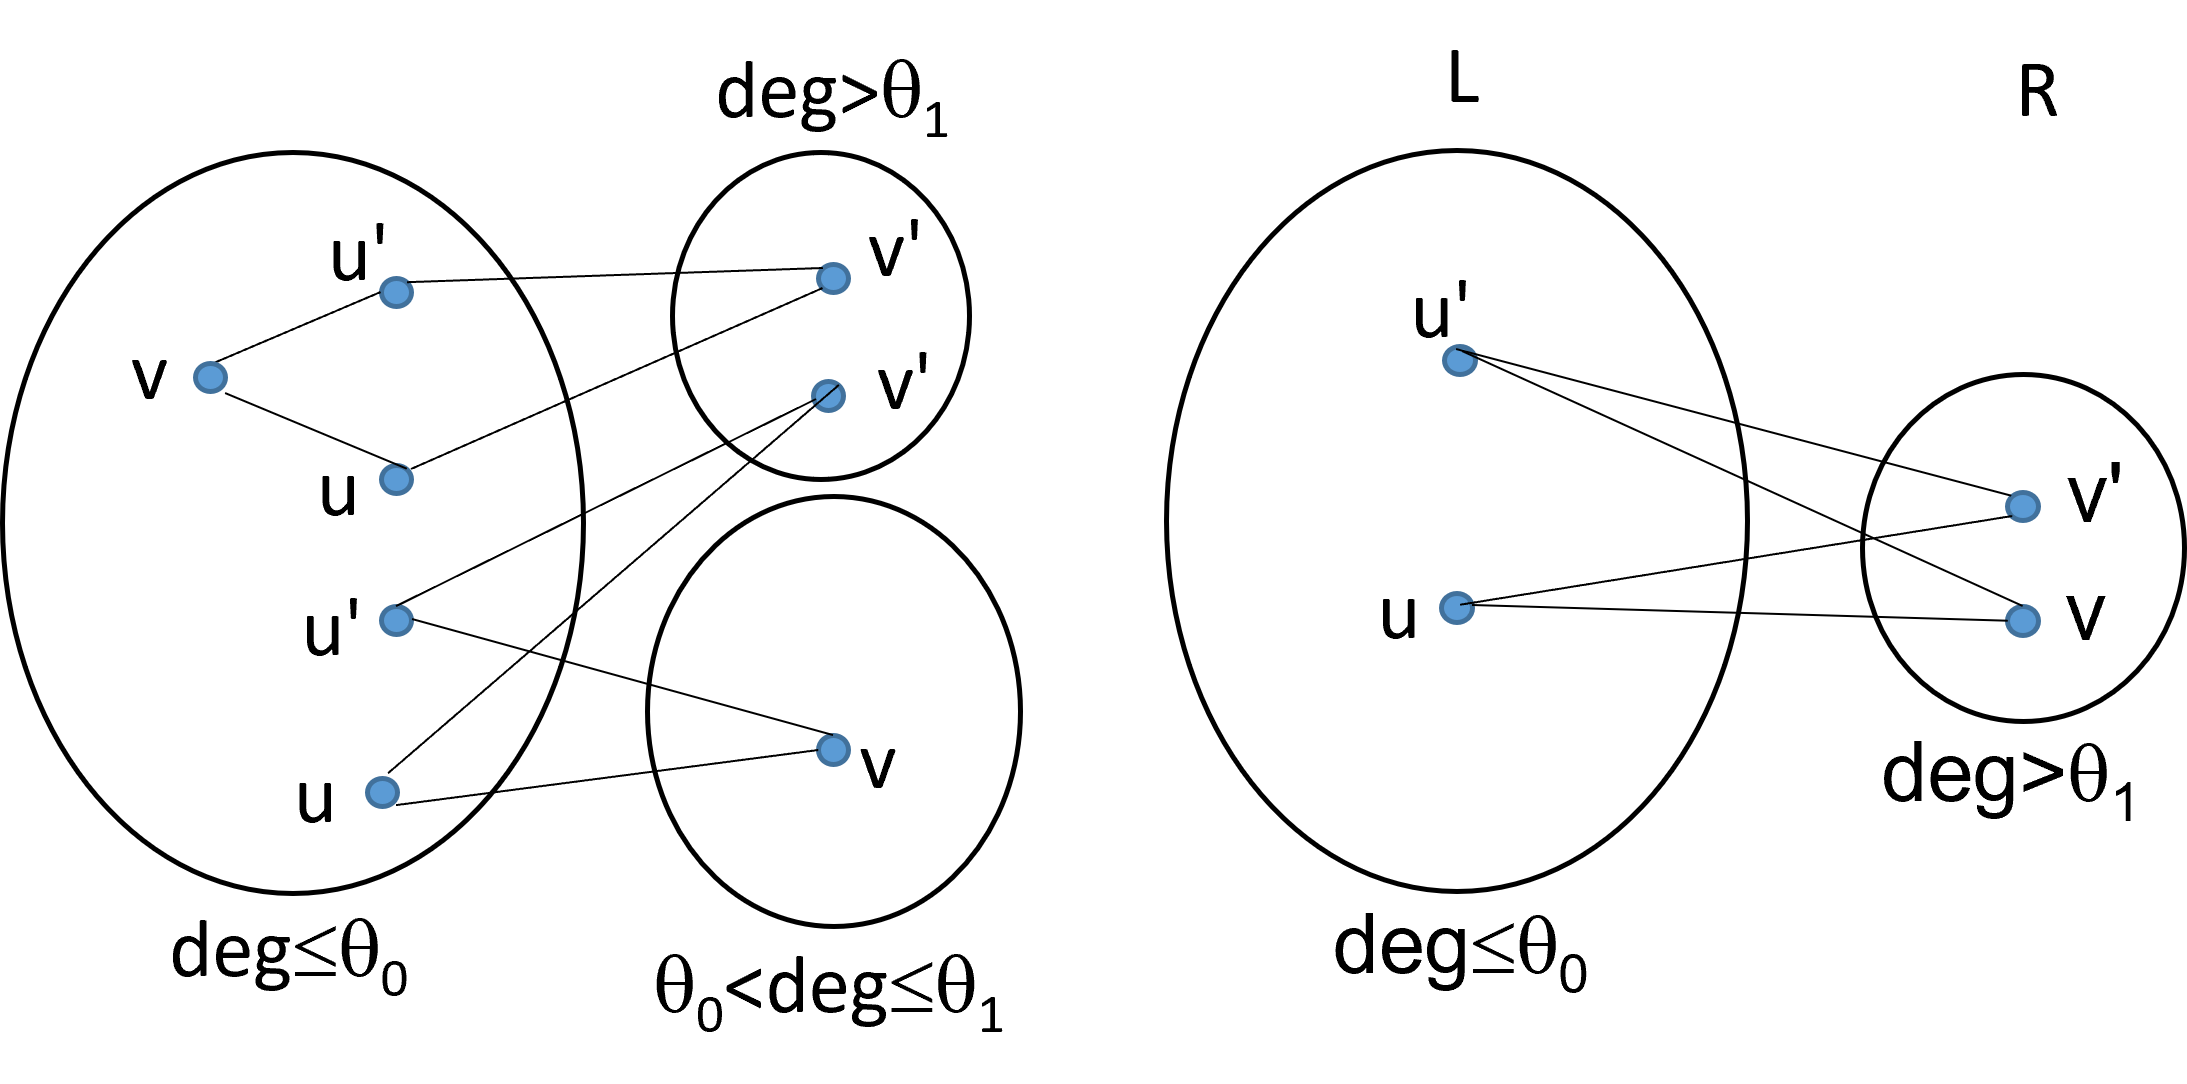
\includegraphics[width=0.5\textwidth]{C4-ub-fig.png}}}
\caption{An illustration for some of the cases considered in the analysis of the algorithm for $C_4$-freeness. On the left side are two examples in which there is a single vertex $v'$ with degree greater than $\theta_1$, so that there is a vertex $v$ with degree at most $\theta_1$ with two neighbors whose degree is at most $\theta_0$.
On the right is an illustration when there are two such vertices with degree greater than $\theta_1$.}
\label{fig:C4-ub}
\end{figure}


\smallskip\noindent\textsf{$C_4$s with two high-degree vertex.}
We now turn to the case in which $|\calC_2| = \Omega(m)$.
Here too we can show that there exists a subset of $\calC_2$, denoted $\calC_2'$, such that $|\calC_2'|=\Omega(m)$, and every vertex $v$ that participates in one of the $C_4$s in $\calC_2'$ actually participates in $\Omega(d(v))$ edges-disjoint $C_4$s in $\calC_2$. 

Recall that by the definitions of $\calC$ and $\calC_2$ and since $\calC_2'\subseteq \calC_2\subseteq \calC$, the following holds. For each $4$-cycle $\rho$ in $\calC_2'$, since it is in $\calC_2$, there are two vertices whose degree is greater than $\theta_1$. Therefore, by the definition of $\calC$, they are both adjacent on $\rho$ to two vertices whose degree is at most $\theta_0$. Hence, if we consider the subgraph induced by the vertices and edges of the $C_4$s in $\calC_2'$, it is a bipartite graph, where on one side, denoted $L$, all vertices have degree at most $\theta_0$, and on the other side, denoted $R$, all vertices have degree greater than $\theta_1$. Furthermore, by the definition of $\calC'_2$, for each vertex in $R$, a constant fraction of its neighbors (in the original graph $G$) belong to $L$, and for each vertex in $L$, a constant fraction of its neighbors belong to $R$. For an illustration, see the RHS of Figure~\ref{fig:C4-ub}. 

Hence, if we select an edge almost uniformly and pick one of its endpoints with equal probability, with high constant probability we obtain a vertex $v\in R$. Conditioned on this event, since $d(v)> \theta_1$, the algorithm will perform $\widetilde{O}(n^{1/4}\alpha^{1/2})$ random walks of length two from $v$, and with high constant probability, a constant fraction of these walks will be of the form $(v,u,v')$ where $u\in L$ and $v' \in R$.
If for some $v'$ we get two walks, $(v,u,v')$ and $(v,u',v')$ for $u \neq u'$, then a $C_4$ is detected.

Observe that since all vertices in $R$ have degree greater than $\theta_1 = \Theta(n^{1/2})$, we have that $|R| \leq 2m/\theta_1 = O(n^{1/2}\alpha)$. This can be used to show that the expected number of pairs of walks that induce a $C_4$ is greater than $1$. In order to show that we actually get such a pair with high constant probability, we perform a more careful analysis to bound the variance. 


%%%%%%%%%%%%%%%%%%%%%%%%%%%%%%%%%%
\iffalse
In order to detect a $C_4$, we consider the following hypothetical process, which removes at most $\eps m$ edges (and hence at most $\eps m$ edge-disjoint $C_4$'s) from the graph. 
We start with a maximal set of $C_4$s in $G$, denote $\calC$, so that $\calC>\eps m$.
First, we remove all edges between vertices with degree greater than  $2c'\alpha/\epsilon$. Since the graph has arboricity $\alpha$, this results in removing at most $\eps m/c'$ edges (and $C_4$'s from $\calC$).  Now in  $\calC$  there are only left $C_4$'s with either at most one, or exactly two vertices with degree greater than $\theta$. \commentt{introduce $\theta$} Let $\calC_1$ denote the former type, and $\calC_2$ the latter. Since these sets are disjoint, it holds that at least one of these sets is of size greater than $\eps m/16$ (as their union is greater than $\eps m/4$).

\paragraph{$C_4$s with one high degree vertex}
We first consider the case that $|\calC_1|>\eps m/16$, and continue the edge removal process: we remove all edges incident to vertices $v$ whose number of $C_4$s in $\calC_1$ is less than $\eps d(v)/64$. Since this process removes at most $\eps d(v)/32$ edges from $G$, at the end of it, we have that the in  ``surviving'' set of $C_4$s in $\calC_1>$, denote $\calC_1'$, there are more than $\eps m/32$ four-cycles. By the construction of this set, each four-cycle $C=(v,v_1, v_2, v_3)$ in $\calC_1'$ 
have at most one vertex, w.l.o.g. $v_2$,  with degree greater than  $\theta$, and at least two vertices, w.l.o.g. $v_1,v_3$ with degree at most $d'$ (so that $v_1$ potentially has degree more than $d'$, but no more than $\theta$).
Furthermore,  \emph{all} of the vertices in each $C_4$ have at least $\eps/64$ of their edges incident to $C_4$s in $G$.  In each $C_4$  in $\calC_1$ ``color'' the vertex that is across from the highest degree vertex blue. 
We try to detect a $C_4$ in $\calC_1$ by trying to first  sample  a blue vertex $v$, and then perform sufficiently many length-2 random walks starting from it, so that with high probability, at least two of them collide on the end vertex. 

To select a blue vertex, the algorithm first selects 
$\Theta(1/\eps)$ edges 
from the set of edges incident to vertices with degree at most $d'$ (by performing  $\Theta(\alpha/(d'\cdot \eps))$ \talya{verify}  many queries),   and then selects one of the sampled edges endpoints u.a.r.. This results in a blue vertex $v$ being selected with high probability. Conditioned on the event that we sampled a blue vertex $v$, we have that $\eps d(v)/64$ of its incident edges participate in $C_4$ in $\calC_1$. Therefore, it has $\eps d(v)/128$ \emph{pairs} of incident edges such that both belong to the same $C_4$. Hence, by taking $\Theta(\sqrt{d(v)/\eps})$ \talya{verify} length-2 random walks from $v$, at least for one pair in the set of walks, both walks starts at edges that belong to the same four-cycle $C=(v, v_1, v_2, v_3)$ in $\calC_1$. Since by definition of $C_1$, all other vertices in $C$ (i.e, all but $v$) have degree at most $d'$, the probability that the second step in each of this walks reaches $v_3$ is at least $1/(d')^2$. Putting everything together, and using a birthday type argument (Corollary~\ref{cor:cheb1}), it can be shown that taking $\Theta(\sqrt{d(v)/\eps}\cdot d')$ many length-2 random walks from each of the $O(1/\eps)$ selected  ``potential'' blue vertices, results in a $C_4$ with high probability. Hence, the total query complexity is $O(\sqrt{d(v)/\eps}\cdot d'\cdot (1/\eps)=O(n^{1/4}\cdot \alpha/\eps^{2.5})$.\talya{verify} 


\paragraph{$C_4$s with two high degree ($>\theta$) vertices}
We now consider the case that $\calC_2$ is of size $\eps m/16$, where recall that in each  $C=(v,v_1,v_2,v_3)\in \calC_2$, there are two vertices, w.l.o.g $v, v_2$ with
degree greater than $\theta$ that do not neighbor each other on the $C_4$, and there are two vertices $v_1,v_3$ with degree at most $d'$ that each neighbors both $v$ and $v_3$. Here too  we remove all edges incident to vertices $v$ whose number of vertices in $\calC_1$ is less than $\eps d(v)/64$.
\fi
%%%%%%%%%%%%%%%%%%%%%%%%%%%%%%%%%%%%%%%%


\paragraph{A (two-sided error) lower bound for testing $C_4$-freeness in constant arboricity graphs.}
To obtain %our first lower bounded, which is for constant arboricity graphs and two-sided error algorithms, 
this lower bound \ICALPCR{of $\Omega(n^{1/4})$},
we define two distributions over graphs.
In the support of the first distribution, $\calD_0$, all graphs are $C_4$-free, and in the support of the second distribution, $\calD_1$, all graphs are $\Omega(1)$-far from being $C_4$-free. Furthermore, $\calD_0$ is uniform over all graphs isomorphic to a specific  graph $G_0$, and $\calD_1$ is uniform over all graphs isomorphic to a specific graph $G_1$.

We next describe a slightly simplified version of the two graphs (which cannot be used to prove the lower bound, but gives the essence of the proof). Both graphs are bipartite graphs, where one side, $Y$, contains $\Theta(\sqrt{n})$ vertices, and the other side, $X$, contains $\Theta(n)$ vertices, In $G_0$, each vertex in $X$ has a unique pair of neighbors in $Y$ (so there are no $C_4$s). On the other hand, in $G_1$, each vertex $x$ in $X$ has a ``twin'', $x'$, where $x$ and $x'$ have the same pair of neighbors in $Y$ (thus creating $\Omega(n)$ edge-disjoint $C_4$. See Figure~\ref{fig:C4-lb}.
\ICALPCR{Observe that the arboricity of both graphs is $2$ as for any subset of vertices $S$, the number of edges within $S$ is at most $|S\cap X| \cdot 2$ so the average degree in the subgraph induced by $S$ is at most $2$.}

In order to prove that no (possibly adaptive) algorithm can distinguish between a graph selected according to $\calD_0$ and a graph selected according to $\calD_1$, we define two processes, $\calP_0$ and $\calP_1$, which answer the queries of a testing algorithm while selecting a graph from $\calD_0$ (respectively, $\calD_1$) ``on the fly''.
The lower bound of $\Omega(n^{1/4})$ follows from the fact that when performing 
% these many queries, 
\SodaReb{fewer than $n^{1/4}/c$ queries (where $c$ is a sufficiently large constant),}
for both distributions, with high constant probability, each new neighbor query is answered by a uniformly selected vertex id.

\begin{figure}[htb!]
\centerline{\mbox{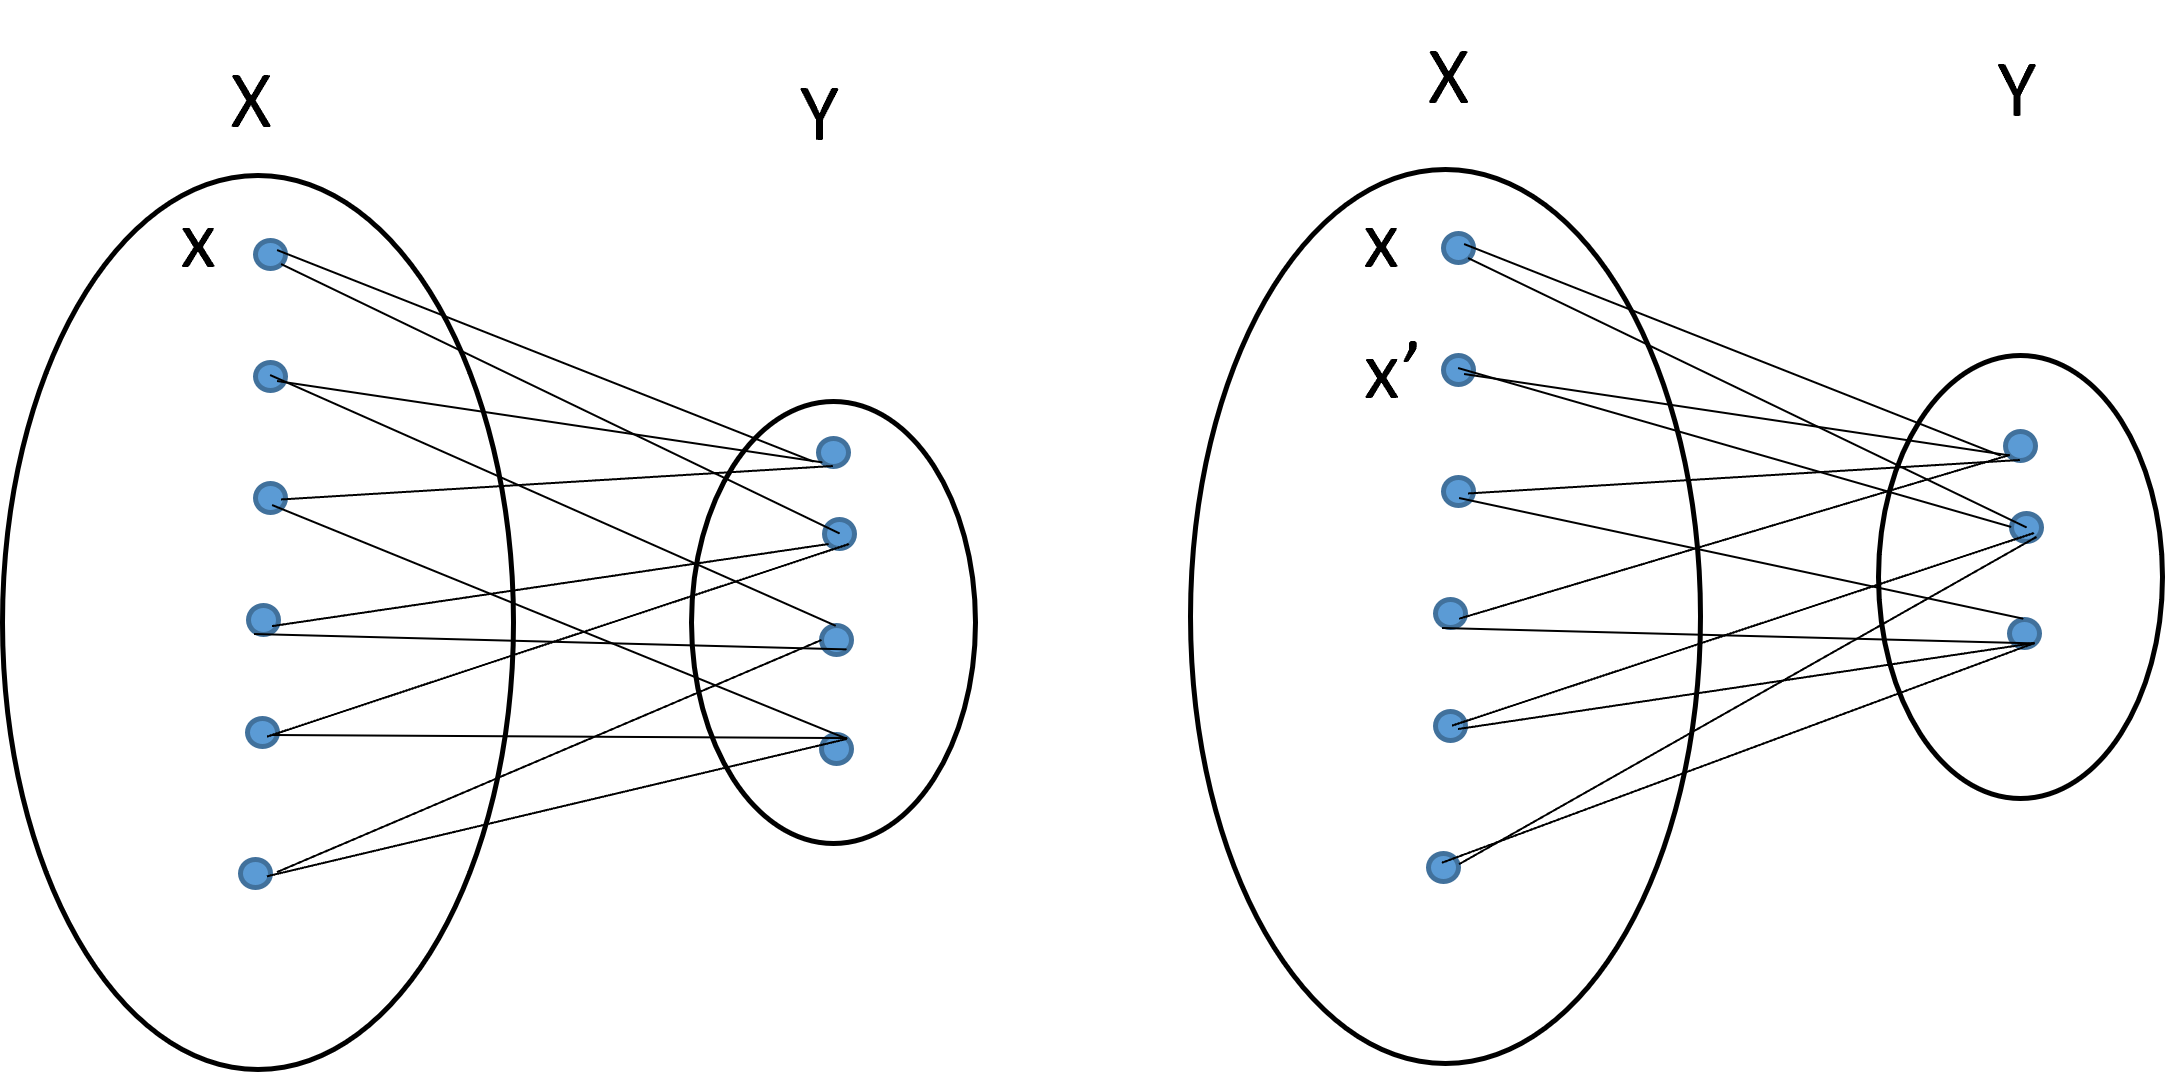
\includegraphics[width=0.5\textwidth]{C4-const-arb-lb.png}}}
\caption{An illustration for the lower bound construction. The graph on the left is $C_4$-free while the graph on the right contains $\Omega(m)$ edge-disjoint $C_4$s and is hence $\Omega(1)$-far from being $C_4$-free.}
\label{fig:C4-lb}
\end{figure}


\paragraph{A one-sided error lower bound for testing $C_4$-freeness in graphs with arboricity $\mathbf{\alpha}$.}
We next  discuss the lower bound of $\Omega(n^{1/4}\alpha^{1/2})$ for graphs with arboricity $\alpha = \Omega(\log n)$ and one-sided error algorithms. 

Here we define a single distribution $\calD$ which is uniform over a family of graphs with arboricity $\alpha$ such that almost all graphs in this family are $\Omega(1)$-far from $C_4$-free.
%Here too, for the sake of the presentation, we describe a simplified version of the distribution.

Roughly speaking, the graphs in the support of $\calD$ are random bipartite graphs, where one side, $Y$, is of size $\Theta(\sqrt{n}\alpha)$ and the other side, $X$, is of size $\Theta(n)$. Every vertex in $X$ has $\alpha$ neighbors in $Y$, and every vertex in $Y$ has $\Theta(\sqrt{n})$ neighbors in $X$. We need to show that if we select such a graph randomly, then on one hand it will be $\Omega(1)$-far from $C_4$-free, and on the other hand, in order to detect a $C_4$, any algorithm must perform $\Omega(n^{1/4}\alpha^{1/2})$ queries.


We next discuss the high-level idea as to why the resulting graphs are (with high constant probability) far from being $C_4$-free. Consider a fixed edge $(x,y)$ in the bipartite graph, where $x\in X, y\in Y$. The number of $C_4$s this edge participates in is determined by the number of edges between the sets of neighbors of $x$ and $y$, respectively $\Gamma(x)$ and $\Gamma(y)$. Recall that $x$ has $\Theta(\alpha)$ neighbors and $y$ has $\Theta(\sqrt n)$ neighbors. Since overall there are $|X|\cdot |Y|=\Theta(n^{3/2}\alpha)$ potential pairs in the bipartite graph, and $\Theta(n\alpha)$ edges, each pair in $X \times Y$ is an edge with probability $\Theta(1/\sqrt n)$. Hence, the expected number of edges between $\Gamma(x)$ and $\Gamma(y)$ is $|\Gamma(x)| \cdot |\Gamma(y)| \cdot (1/\sqrt n)=\Theta(\alpha)$. By analyzing the variance between pairs of edges, we  furthermore show that with high constant probability, most edges do not participate  in too many $C_4$s. Combining the two insights, it follows that with high constant probability, the graph is indeed far form being $C_4$-free.

 
In order to prove that any algorithm that performs at most  $n^{1/4}\alpha^{1/2}/c$   queries (for a sufficiently large constant $c$), will not detect a $C_4$ with high constant probability, we actually prove that it will not detect \emph{any} cycle.  Roughly speaking, we show that by the randomness of the construction, 
since $|Y|=\Theta(\sqrt n \alpha)$, and the algorithm performs $O(\sqrt{|Y|})$ queries,
each new neighbor query is answered by a uniformly   distributed vertex that has not yet been observed. Therefore, the algorithm essentially views a forest. 



A central challenge that we need to overcome is that we do not want to allow parallel edges, where the above construction might lead to their existence. One possibility is to first define the distribution over graphs with parallel edges and then to remove them. The benefit is that due to the higher degree of independence in the construction, it is somewhat easier to formally prove that the graphs obtained (with parallel edges) are with high probability $\Omega(1)$-far from $C_4$-free, and this remains the case when we remove parallel edges.

However, this creates a 
%\commentt{removed "serious technical'' since somehow sounded too serious..}
% serious technical 
difficulty when we turn to argue that no (one-sided error) algorithm can detect a $C_4$ unless it makes $\Omega(n^{1/4}\alpha^{1/2})$ queries. The difficulty is due to the fact that % our model allows degree queries, and so 
in the formal proof we need to deal with dependencies that arise due to varying degrees (which occur because parallel edges are removed). While intuitively, varying degree should not actually ``help'' the algorithm, this intuition is difficult to formalize.
Hence, we have chosen to define the distribution, from the start, over graphs that do not have parallel edges.
This choice creates some technical challenges of its own (in particular in the argument that the graphs obtained are $\Omega(1)$-far from $C_4$-free), but we are able to overcome them. For the full details see Section~\ref{sec:C4-lb}.


%\subsubsection*{The improved upper bound for $C_4$-freeness}
%\subsubsection*{The lower bounds for $C_4$-freeness}


\subsubsection{The algorithm for $C_6$-freeness}
\ICALPCR{Recall that for $C_6$ we have a (one-sided error) testing algorithm whose query complexity is $\widetilde{O}(n^{1/2})$.}
In addition to assuming (for the sake of the exposition) that $\eps$ is a constant, we also 
ignore polylogarithmic factors in $n$. Similarly to the algorithm for testing $C_4$-freeness, the algorithm for testing $C_6$-freeness, \TestCsix,  in constant arboricity graphs is governed by two thresholds. The first, $\theta_0$, is of the order of the arboricity, so that it is a constant (recall that we assume that $\eps$ is a constant). The second, $\theta_2$, is of the order of $\sqrt{n}$.

The algorithm repeats the following process several times. It selects a vertex $v$ uniformly at random, and if $d(v) \leq \theta_0$, it performs a \emph{restricted} BFS starting from $v$ to depth $4$. Specifically:
\begin{packed_enum}
           \item Whenever a vertex $u$ is reached such that $d(u) \leq \theta_0$, all its neighbors are queried.
           \item Whenever a vertex $u$ is reached such that $d(u) > \theta_0$ and $u$ is reached from a vertex $u'$ such that $d(u') \leq \theta_0$, there are two sub-cases. If $d(u) \leq \theta_1$, then  all of $u$'s neighbors are queried. Otherwise,  $\theta_1$ neighbors of $u$ are selected uniformly at random. \label{step:C6_rand_nbr}
               %\commentt{Or should we use $\ell$ here?}
           \item Whenever a vertex $u$ is reached from a vertex $u'$ such that both $d(u)>\theta_0$ and $d(u') > \theta_0$, the BFS does not continue from $u$.
\end{packed_enum}
         
 % whenever a vertex $u$ is reached such that $d(u) \leq \theta_0$, all its neighbors are queried, and the same holds when a vertex $u$ is reached such that $\theta_0 < d(u) \leq \theta_1$ conditioned on $u$ being reached from a vertex $u'$ such that $d(u') \leq \theta_0$. If $d(u) > \theta_1$, but it is reached from $u'$ such that $d(u') \leq \theta_0$, then $\theta_1$ random neighbors of $u$ are selected. Otherwise ($d(u)> \theta_0$ and it is reached from $u'$ such that $d(u')>\theta_0$, the BFS does not continue from $u$. Hence, the number of queries performed in such a restricted BFS is $O(\sqrt{n})$.
The algorithm rejects if and only if it observes a $C_6$.

Consider a graph that is far from being $C_6$-free, so that it contains a set  of $\Omega(m)=\Omega(n)$ edge-disjoint $C_6$s. Furthermore, it contains such a set, denoted $\calC$ for which every $C_6$ in $\calC$ contains at most three vertices with degree greater than $\theta_0$, and furthermore, these vertices are  \emph{not} adjacent on the $C_6$. We partition $\calC$ into three subsets: $\calC_1$, $\calC_2$, and $\calC_3$, depending on the number of vertices with degree greater than $\theta_0$ that it contains.

If either $|\calC_1| = \Omega(m)$, or $|\calC_2| = \Omega(m)$, then it is not hard to show that the algorithm will detect a $C_6$ with high constant probability. The more interesting part of the proof is handling the case in which only $|\calC_3| = \Omega(m)$.

In this case we define an auxiliary multi-graph, denoted $G'$, over the set of vertices that participate in $C_6$s belonging to $\calC_3$, and have degree greater than $\theta_0$ (in $G$). We denote this set of vertices by $M$, and the set of vertices with degree at most $\theta_0$ that participate in these $C_6$s, by $L$. 

Assume for simplicity that each vertex in $L$ has degree exactly $2$ (i.e., it participates in a single $C_6$).
For each pair of vertices in $M$, we put in $G'$ a set of parallel edges, whose size equals the number of  length-2 paths between them in $G$ that pass through vertices in $L$.
Hence, for each $C_6$ in $\calC$, we have a triangle in $G'$, where these triangles are edge-disjoint, and we denote their set by $\calT$. See Figure~\ref{fig:C6}.

\begin{figure}[htb!]
\centerline{\mbox{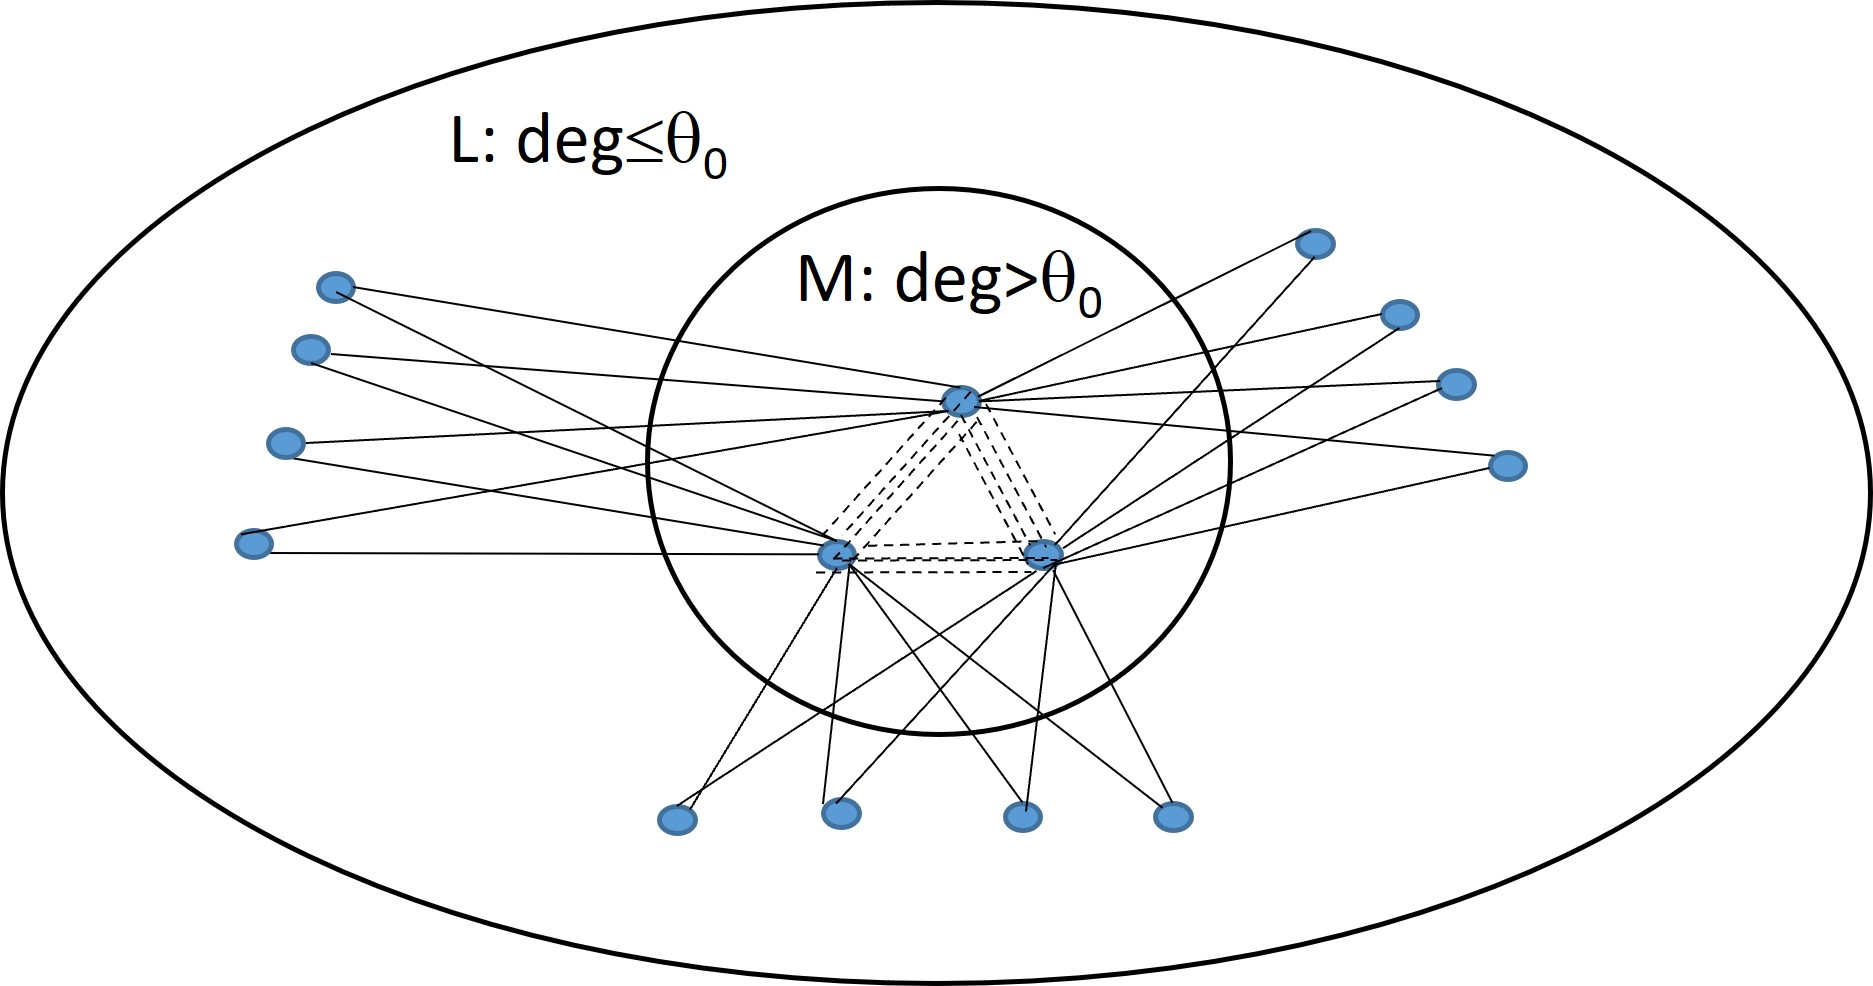
\includegraphics[width=0.5\textwidth]{C6fig.jpg}}}
\caption{An illustration of the auxiliary (multi-)graph $G'$ in the $C_6$-freeness testing algorithm. The dashed lines represent edges in $G'$, each one corresponding to a length-2 path in $G$ that passes through a vertex with degree at most $\theta_0$.
% \talya{check caption}} \commentt{added a few more words - this is not exactly the construction, but close enough)
}
\label{fig:C6}
\end{figure}


Observe that selecting a vertex uniformly at random from $L$ 
and querying its two neighbors in $M$ 
corresponds to selecting an edge uniformly at random in $G'$. If we add an additional simplifying assumption by which (in $G$), vertices belonging to $M$ only neighbor vertices belonging to $L$, then our algorithm on $G$ essentially translates to picking a random edge in $G'$. Then depending on the degree of the endpoints, either querying all their neighbors in $G'$ or $\theta_1$ random neighbors. 

Let $H$ denote the subset of vertices in $M$ whose degree in $G$ is greater than $\theta_1$.
If relatively many triangles in $\calT$ contain at most
one vertex in $H$, then we are done, since these triangles contain an edge for which  both endpoints have degree at most $\theta_1$.
Hence, it remains to address the case in which almost all triangles in $\calT$ have two or three vertices in $H$.

Roughly speaking, in this case we show that the existence of many edge-disjoint, but not vertex-disjoint, 
 triangles in $G'$ that contain such high-degree vertices  implies the existence of ``many more'' triangles that may be caught by our algorithm. As an illustrative extreme (but easy) special case, assume that in $G'$ there are only three vertices. Then the existence of some number $t$ of edge-disjoint triangles between them, actually implies the existence of $t^3$ (non edge-disjoint) triangles.


\subsubsection{The general lower bound %of $\Omega(n^{1/3})$ 
   for $C_k$-freeness, $k\geq 6$}
We establish our general lower bound \ICALPCR{of $\Omega(n^{1/3})$}
for one-sided error testing of $C_k$-freeness when $k\geq 6$ by %reducing from 
building on a lower bound for testing triangle-freeness that appears in~\cite[Lemma 2]{AKKR08}. This lower bound on testing triangle-freeness is based on the difficulty of detecting a triangle in graphs selected uniformly from a family $\mG_{\trn}$ of graphs %over $\trn$ vertices 
in which almost all graphs are $\Omega(1)$-far from being triangle-free. All graphs in the family are $d$-regular tri-partite graphs over $\trn$ vertices and the lower bound on the number of queries necessary to detect a triangle (with constant probability), is $\Omega(\min\{d,\trn/d\})$. By setting $d= \sqrt{\trn}$, the lower bound is $\Omega(\sqrt{\trn})$.

We show that, for any constant $k\geq 6$, if we had a one-sided error testing algorithm $\mA$ for  $C_k$-freeness of graphs with $n$ vertices and constant arboricity using at most $n^{1/3}/c$ queries (for a constant $c$), then we would be able to detect triangles in graphs selected uniformly from $\mG_{\trn}$ using at most $\sqrt{\trn}/c'$ queries (for a constant $c'$). 


To this end we define an algorithm $\mA$ that, given query access to a graph $\trG \in \mG_{\trn}$, implicitly defines a graph $G$ for which the following holds. First, the number of vertices in $G$ is $n=\Theta({(\trn)}^{3/2})$, and the number of edges is $m = \Theta(\trm)$, where $\trm$ is the number of edges in $\trG$ (so that $\trm = \Theta((\trn)^{3/2})$). Second, $G$ has arboricity $2$. Third, the distance of $G$ to $C_k$-freeness is of the same order as the distance of $\trG$ to triangle-freeness. Fourth, there is a one-to-one correspondence between triangles in $\trG$ and $C_k$s in $G$. The basic idea is to replace edges in the tri-partite graph $\trG$ with paths of length $k/3$. See Figure~\ref{fig:gen-lb}


\begin{figure}[h!]
\centerline{\mbox{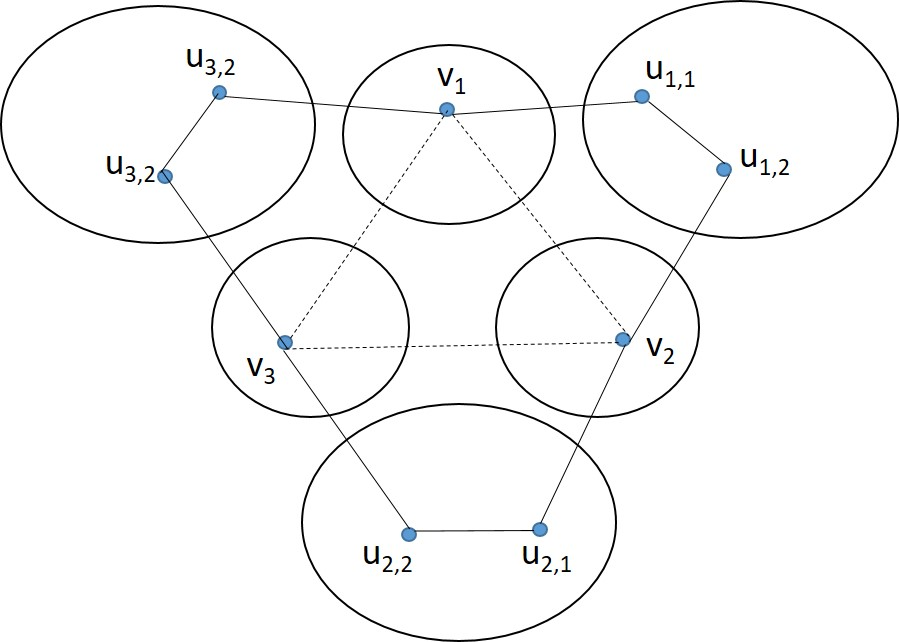
\includegraphics[width=0.4\textwidth]{gen-lb-fig.jpg}}}
\caption{An illustration for the lower bound construction for $C_k$-freeness in constant arboricity graphs when $k=9$.
The three circles in the middle and the dashed lines represent a graph $G'\in \calG_{n'}$. The outer circles represent the additional vertices in $G$. Since $k=9$ in this example, each edge in $G'$ is replaced by a path of length 3 in $G$.
}
\label{fig:gen-lb}
\end{figure}


Assuming there existed a testing algorithm $\mA$ as stated above, the algorithm $\trA$ would use it to try and find a $C_k$ in $G$ (and hence a triangle in $\trG$). In order to be able to run $\mA$ on $G$, the algorithm $\trA$ must be able to answer queries of $\mA$ to $G$ by performing queries to $\trG$. We show how this can be done with  a constant multiplicative overhead.
Hence, the lower bound of $\Omega(\sqrt{\trn})$ for testing triangle-freeness (when the degree is $\Theta(\sqrt{\trn})$) translated into a lower bound of $\Omega(n^{1/3})$ for testing $C_k$-freeness.



\subsubsection{The general upper bound for  $C_k$-freeness}
%\commentt{made some changes, please see what you think}
% Here too we assume for the sake of the exposition that $\eps$ is a constant, and 
Recall that our starting point is that if $G$ is $\Omega(1)$-far from being $C_k$-free, then it contains a set $\calC$ of $\Omega(m)$ edge-disjoint $C_k$'s that do not contain any edge between vertices that both have degree greater than $\theta_0 = \Theta(\alpha)$. We refer to vertices with degree at most $\theta_0$ as \emph{light} vertices, and to those with degree greater than $\theta_0$ as \emph{heavy}.
Hence, each $C_k$ in $\calC$ has at least $\lceil k/2\rceil$ light vertices, and each heavy vertex
on it neighbors two light vertices.

We present two different algorithms, where each of them is suitable for a different setting. The basic idea of both algorithms is to take a large enough sample of vertices and edges so that the  subgraph determined by 
the sampled light vertices and their incident edges, as well as the sampled edges, contains a copy of $C_k$. \ICALPCR{The query complexity of each algorithm is stated following its high-level description.}

\paragraph{The first algorithm.}
Our first algorithm simply samples vertices uniformly, independently at random, and then performs queries that reveal the neighbors of all light vertices in the sample.
To analyze what is the sufficient sample size for this algorithm, consider the following generalization of the birthday paradox for $k$-way collisions. Assume we sample elements under the uniform distribution over $[n]$. Then we obtain a $k$-way collision after taking $\Theta(n^{1-1/k})$ samples.
Similarly, suppose  we sample vertices uniformly from a graph that is composed only of $n/k$  vertex-disjoint copies of $C_k$. Then, after sampling $\Theta(n^{1-1/k})$ vertices, we will hit all the vertices of at least one of the copies (with high constant probability).
Conditioned on this event, if we reveal the neighborhood of all the vertices in the sample, then  we obtain a $C_k$.

The next observation is that, in fact, we only need to hit a \emph{vertex cover} of a copy of a $C_k$ (as opposed to all its vertices). In particular we would like to hit such a cover that contains only light vertices, which we refer to as a \emph{light vertex cover}. 
For constant $\alpha$, this yields an improved dependence on $k$ in the exponent, i.e., $O(n^{1-1/\lfloor k/2\rfloor})$ sampled vertices suffice.
% This yields an improved dependence in the exponent. \reut{The improved for constant $\alpha$ and $\epsilon$ }
% \reut{change terms}
%

When taking into account the dependence on $\alpha$ (so that it is not necessarily true that $m=O(n)$) and incorporating this in the analysis, we prove that the query complexity is upper bounded by $O(m \cdot (\alpha/m)^{2/k})$ for even $k$ and $O(m \cdot (\alpha/m)^{2/(k+1)})$ for odd $k$ 
(up to a polynomial dependence on $k$).
% \reut{(up to polynomial dependence in $k/\epsilon$)}.
%\reut{change in abstract and intro ceiling to floor} \commentt{changed}
Since $\alpha \leq \sqrt{m}$ it follows that the above bounds are at most $O(m^{1-1/k})$ and $O(m^{1-1/(k+1)})$, respectively. 

\paragraph{The second algorithm.}
Our second algorithm is designed for the case in which $k$ is odd and $m = \Omega(\alpha^{(k+3)/2})$. In particular it is preferable when $\alpha$ is constant. 
We observe that when $k$ is odd, for each $C_k$ in $\calC$, there is an edge in 
 which both endpoints are light vertices.
 \SodaReb{Therefore, if we sample edges (almost) uniformly from the graph (using a variant of the procedure \SelectEdge), then} we are likely to hit one of these edges. This additional step reduces the number of vertices we need to hit in each copy by $2$, which  results in improved complexity for some range of the parameters. In particular, the query complexity of this algorithm is $O(m \cdot (\alpha^2/m)^{2/(k-1)})$.
 %\reut{should be $\alpha$ when k = 3, check why not}
 Specifically, when $\alpha$ is a constant, the query complexity of this algorithm (which works for odd $k$) is $O(m^{1-2/(k-1)})$ (instead of $O(m^{1-2/(k+1)})$).

 \paragraph{General subgraph $F$.}
 Our first algorithm also works for any constant-size subgraph, $F$, where the upper bound on the sample size is of the form $m^{1-1/\ell(F)}$ where $\ell(F)$ depends on the structure of $F$, and is at most $k=|V(F)|$.
% the specific dependence in the size of $F$ in the exponent depends on the structure of $F$\reut{phrasing}. 
 The idea is that if we want to find a copy of $F$, it suffices to hit a light vertex cover of this copy and then query all neighbors of the sampled light vertices. 
 % To this end we define a parameter of $F$ which bounds the number of vertices we need to hit from each copy. This bound is clearly bounded by the number of vertices of $F$ so for any $F$ we obtain a bound of $m^{1-1/|V(F)|}$ queries.
 % (up to polynomial dependence on $|V(F)|/\epsilon$).

% \commentt{Depending on what we do with $C_5$, this subsection might be for both $C_5$ and $C_6$ -- I think that the complexity of $C_5$ for constant arboricity is the same as for $C_4$, but the algorithm and analysis might be more similar to $C_6$ (unless we are able to get a reduction, which we weren't able to get in the past}



\subsection{Related work}\label{subsec:related}
In this subsection we shortly discuss several related works, in addition to the two aforementioned works regarding testing $C_3$-freeness~\cite{AKKR08,Reut}.

Testing subgraph-freeness for fixed, constant size subgraphs in the dense-graphs model can be done using a number of queries that depends only on $1/\eps$ (where the dependence is a tower of height $\poly(1/\eps)$), as shown by Alon, Fischer, Krivelevich and Szegedy~\cite{AFKS00}.  Alon~\cite{Alo02} proved that a super polynomial dependence on $1/\eps$ is necessary, unless the subgraph $F$ is bipartite. Goldreich and Ron addressed the problem in the bounded-degree model~\cite{GR-bound}, and gave a simple algorithm that depends polynomially on $1/\eps$ and the maximum degree in the graph, and exponentially on the diameter of $F$.

A special case of graphs that have bounded arboricity is the family of graphs that exclude a fixed minor (a.k.a. minor-free graphs).
%Benjamini, Schramm and Shapira~\cite{BSS08} 
Newman and Sohler~\cite{NS13} showed that 
for this family of graphs, in the bounded-degree model, all properties 
% testing $F$-freeness  with one sided-error can be done 
can be tested with no dependence on the size of the graph $G$. Moreover, it was recently shown~\cite{SS21,LS21} that any property which is monotone and additive\footnote{A property is monotone if it closed under removal of edges and vertices. A property is 
additive if it is closed under the disjoint union of graphs.} (and in particular $F$-freeness where $F$ is a connected graph) can be tested using a number of queries that is only polynomial in $1/\eps$ and $d$, where $d$ is the degree bound (and $O(d^{\rho(\eps)})$ in general $(\eps, \rho(\eps))$-hyperfinite graphs\footnote{Let $\rho$ be a function from $\mathbb{R}_+$ to $\mathbb{R}_+$. A graph $G = (V, E)$ is $(\eps, \rho(\eps))$-hyperfinite if for every $\epsilon > 0$ it is possible to
remove $\eps |V|$ edges of the graph such that the remaining graph has connected components of size at most $\rho(\eps)$.}).
For minor-free graphs with unbounded degrees, Czumaj and Sohler~\cite{CS19} showed that a property is testable 
%\commentt{what exactly is their definition of ``testable''? is it that it does not depend on the size of the graph but may have an arbitrary dependence on $1/\eps$?}
with one sided error and a number of queries that does not depend on the size of the graph if and only if it can be reduced to testing for a finite family of finite forbidden subgraphs.\footnote{They consider a model in which they can perform only random neighbor queries.} The correctness of their algorithm relies on the fact that the arboricity of minor-free graphs remains constant even after contractions of edges (which is not the case for general constant-arboricity graphs). 

In general graphs, it was shown that $k$-path freeness~\cite{IY18} and more generally $T$-freeness where $T$ is a tree of order $k$~\cite{EFFGLMMOORT17}, can be tested with time and query complexity that depend only on $k$, assuming the edges of the graph can be accessed uniformly at random.
Testing cycle-freeness (where a no instance is a graph that is far from being a forest) was studied in the bounded-degree model in~\cite{GR-bound}, where a two-sided error algorithm was given whose query complexity is polynomial in $1/\eps$ and the degree bound. Czumaj  et. al~\cite{CGRSSS14} showed that the complexity of this problem for one-sided error algorithms in the bounded-degree model is $\widetilde{\Theta}(\sqrt{n})$ (for constant $\eps$ -- their algorithm has a polynomial dependence on $1/\eps$), and the algorithm can be adapted to the general-graphs model.

Other sublinear-time graph algorithms 
for counting and sampling (rather than detecting) subgraphs 
that give improved results when the graph $G$ has bounded arboricity include~\cite{ERS19,ERR19,ERS20, ERR22}. 
% \commentt{Other results?}\reut{added the paper about sampling, did not find anything else in sublinear}
% \commentt{so let's do with that}

\subsection{Organization}
We start in Sections~\ref{sec:prel} with some preliminaries. In 
Section~\ref{sec:C4} we give the upper bound for testing $C_4$-freeness. Few details are deferred to Appendix~\ref{sec:4.1}, and the lower bound for testing $C_4$-freeness is given in 
Appendix~\ref{sec:C4-lb}.
% Sections~\ref{sec:C4}, \ref{sec:4.1} and~\ref{sec:C4-lb} we present our results for testing $C_4$-freeness (both the upper and the lower bounds), and 
In Appendix~\ref{sec:C5} we provide the adaptation of the algorithm for testing $C_4$-freeness, to testing $C_5$-freeness (in graphs with constant arboricity). 
Our algorithm for testing $C_6$-freeness (in graphs with constant arboricity) is given in Appendix~\ref{sec:C6-ub}. Our lower bound for one-sided error testing of $C_k$-freeness is proved in Appendix~\ref{sec:Ck-lb}, and the upper bound is given in Appendix~\ref{sec:Ck}.


